\chapter{Pilas}

\section{Definición de Pila}
Una pila (stack en inglés) es una lista ordinal o estructura de datos en la que el modo de acceso a sus elementos es de tipo LIFO (del inglés Last In First Out, último en entrar, primero en salir) que permite almacenar y recuperar datos. Se aplica en multitud de ocasiones en informática debido a su simplicidad y ordenación implícita en la propia estructura. 

La Figura  \ref{fig:pila-representacion} muestra la representación gráfica de una pila con sus operaciones fundamentales de apilar (push en inglés) y desapilar o retirar (pos en inglés.).

La pila es muy útil en situaciones cuando los datos deben almacenarse y luego recuperarse en orden inverso.

\begin{figure}
	\centering\textbf{}
		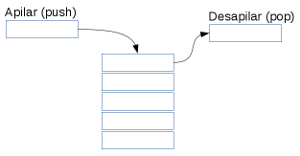
\includegraphics{Diagramas/RepresentacionPila}
	\caption{Representación de una Pila}	
	\label{fig:pila-representacion}
\end{figure}

\begin{definicion}[Pila][capPilas:pila]
Una pila (stack en inglés) es una lista ordinal o estructura de datos en la que el modo de acceso a sus elementos es de tipo LIFO (del inglés Last In First Out, último en entrar, primero en salir) que permite almacenar y recuperar datos. FALTA REFERENCIA
\end{definicion}

\section{El TAD Pila}
A continuación se especifica el TAD de la Pila con sus operaciones fundamentales. Las operaciones apilar y desapilar son las más importantes. En seguida la especificación de cada operación del TAD al estilo C.

\begin{lstlisting}[numbers=none, language=C]
TAD Pila [ T ]
{ invariante: TRUE }
Constructoras:
   crearPila: 
Modificadoras:
	apilar: Pila T 
	desapilar: Pila
Analizadoras:
	cima: Pila 
	esVacia: Pila
Destructora:
	destruirPila: Pila

Pila crearPila( void )
/* Crea una pila vacia */
{ post: crearPila = \phi }

void apilar(Pila pil, T elem)
/* Coloca sobre el tope de la pila el elemento elem */\
{ post: pil = e1, e2, .. elem}

void desapilar(Pila pil)\\
/* Elimina el elemento que se encuentra en el tope de la pila */\\
{ pre: pil =e1, e2, ..en, n > 0 }
{ post: pil =e1, e2, .., en-1 }

T cima(Pila pil )
/* Retorna el elemento que se encuentra en el tope de la pila */
{ pre: n > 0 }
{ post: cima = en }

int esVacia( Pila pil )
/* Informa si la pila esta vacia */
{ post: esVacia = ( pil =  \phi) }

void destruirPila( Pila pil )
/* Destruye la pila retornando toda la memoria ocupada */
{post: pil ha sido destruida }
\end{lstlisting}

\section{Implementación del TAD Pila en Java}
A continuación se muestra una implementación en Java del TAD Pila. Se ha implementado una pila dinámica utilizando nodos enlazados.  Cada nodo almacena un valor y contiene una referencia al siguiente nodo. Supongamos una pila que almacene datos enteros, a la cual se le han aplicado las siguientes operaciones: apilar(10), apilar(35), apilar(12), apilar(7). La Figura \ref{fig:pila-nodos-enlazados} representa cómo quedaría la pila después de apilar en orden los datos 10, 35, 12 y 7. Se puede apreciar que cada nodo almacena un dato y a la vez existe una referencia que almacena la dirección del siguiente nodo. Además, existe una referencia llamada cabeza que apunta al último elemento que entró (en este caso al dato 7).

\begin{figure}
	\centering
	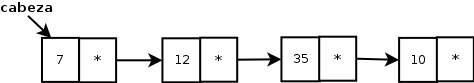
\includegraphics[scale=0.7]{Diagramas/RepresentacionPilaNodosEnlazados}
	\caption{Representación de la Pila con Nodos Enlazados}	
	\label{fig:pila-nodos-enlazados}
\end{figure}

La Figura \ref{fig:pila-diagrama-clases} muestra el diagrama de clases. Se puede apreciar básicamente dos clases: \textit{Nodo} y \textit{Pila}. La clase \textit{Nodo} representa cada uno de los nodos enlazados que almacenan los objetos que se apilan. Tiene dos atributos,  \textsl{valor} que representa el valor que guarda el nodo, en este caso es una referencia a un objetivo de tipo T (siendo T un tipo genérico). El atributo \textsl{siguiente}, representa la referencia al siguiente nodo. Los demás son únicamente, constructor y getters y setters de cada atributo. A continuación el código fuente de la clase Nodo.


\begin{figure}
	\centering
		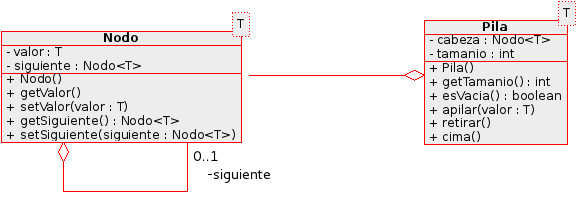
\includegraphics{Diagramas/DiagramaClases-Pila}
	\caption{Diagrama de clase de la implementación del TAD Pila}	
	\label{fig:pila-diagrama-clases}
\end{figure}

\begin{lstlisting}[language=Java]
package co.unicauca.pilas;
public class Nodo<T> {
	//Atributo valor de tipo T. Almacena la referencia al objeto que se guarda en el nodo
 	private T valor;
 	//Referencia al siguiente nodo enlazado
 	Nodo<T> siguiente;
	//Constructor por defecto
 	public Nodo() {
 		valor = null;
 		siguiente = null;
 	}
	//Devuelve el valor 
 	public T getValor() {
 		return valor;
 	}
	//Modifica el valor
 	public void setValor(T valor) {
 		this.valor = valor;
 	}
	//Devuelve el atributo siguiente
 	public Nodo<T> getSiguiente() {
 		return siguiente;
 	}
	 //Modifica el atributo siguiente
 	public void setSiguiente(Nodo<T> siguiente) {
 		this.siguiente = siguiente;
 	}
 }
\end{lstlisting}

La clase \textit{Pila} representa la pila como tal con sus operaciones principales de \textsl{apilar} y \textsl{retirar}. A continuación el código fuente de la clase Pila.

\begin{lstlisting}[language=Java]
package co.unicauca.pilas;
public class Pila<T> {
    //Atributo cabeza, que apunta al tope la pila
 	private Nodo<T> cabeza;
 	//Almacena el total de elemento de la pila
 	private int tamanio;
    //Constructor por defecto
 	public Pila() {
 		cabeza = null;
 		tamanio = 0;
 	}
	//Devuelve el total de elementos de la pila
 	public int getTamanio() {
 		return tamanio;
 	}
	//Verifica si la pila esta vacia
 	public boolean esVacia() {
 		return (cabeza == null);
 	}
	//Apila un elemento nuevo
 	public void apilar(T valor) {
	 	//Crear un nuevo Nodo
 		Nodo<T> nuevo = new Nodo<T>();
	 	//Fijar el valor dentro del nodo
 		nuevo.setValor(valor);
 		if (esVacia()) {
	 		//Cabeza apunta al nodo nuevo
 			cabeza = nuevo;
 		} else {
	 		//Se enlaza el campo siguiente de nuevo con la cabeza
 			nuevo.setSiguiente(cabeza);
 			//La nueva cabeza de la pila pasa a ser nuevo
 			cabeza = nuevo;
 		}
 		//Incrementa el tamanio porque hay un nuevo elemento en la pila
 		tamanio++;
 	}
	//Elimina un elemento de la pila
 	public void retirar() {
 		if (!esVacia()) {
 			cabeza = cabeza.getSiguiente();
 			tamanio--;
. 		}
 	}
	//Devuelve el elemento almacenado en el tope de la pila
 	public T cima() {
 		if (!esVacia())
 			return cabeza.getValor();
 		else
 			return null;
 	}
 }
\end{lstlisting}

En la línea 21 se puede apreciar el método \textbf{apilar}. Este método recibe como parámetro el \textbf{valor} que quiere apilar. Lo primero que se hace es crear un \textit{nuevo} nodo y fijar su valor (lineas 23 y 24). Una vez creado el nodo, se pregunta si la pila es vacía (linea 26). En caso verdadero la referencia \textit{cabeza} apunta al nodo nuevo (linea 28). De lo contrario se enlaza el campo \textit{siguiente} de nuevo con la \textit{cabeza} (linea 31), y finalmente la \textit{cabeza} apunta a \textit{nuevo} (linea 33) para indicar cual fue el último nodo que entró a la pila. Finalmente, la variable \textit{tamanio} se incrementa (indicando que la pila tiene una elemento mas). Por ejemplo si a la pila de la Figura \ref{fig:pila-nodos-enlazados} le aplicáramos la operación apilar(23), nos daría como resultado la pila de la Figura \ref{fig:pila-nodos-enlazados-apilar}.

\begin{figure}
	\centering
	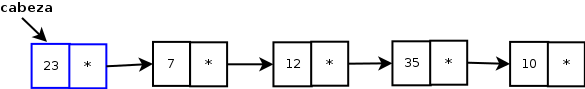
\includegraphics[scale=0.7]{Diagramas/RepresentacionPilaNodosEnlazadosApilar}
	\caption{Representación de la Pila después de apilar el elemento 23}	
	\label{fig:pila-nodos-enlazados-apilar}
\end{figure}

En la linea 39 se aprecia el método \textbf{retirar} (o desapilar). Lo primero que hace es preguntar si la pila no esta vacía (linea 40), en caso afirmativo, la \textit{cabeza} se desplaza al siguiente nodo (linea 41). Finalmente se decrementa la variable \textit{tamanio} (indicando que hay un elemento menos en la pila).

A continuación el código de un Cliente que instancia la Pila que hemos creado. En este caso se almacenan objetos de tipo entero, se apilan algunos números, se imprimen los valores del tope de pila y se desapilan sus elementos.

\begin{lstlisting}[language=Java]
package co.unicauca.pilas;
public class ClienteMain {
	public static void main(String[] args) {
		//Crear una nueva pila de enteros
		Pila<Integer> pila2 = new Pila<Integer>();
		//Se apilan algunos datos enteros
		pila2.apilar(2);
		pila2.apilar(5);
		pila2.apilar(7);
		System.out.println("El tope de la pila es: " + pila2.cima());
		//Se desapila
		pila2.retirar();
		System.out.println("El tope de la pila es: " + pila2.cima());
		//Se desapila
		pila2.retirar();
		System.out.println("El tope de la pila es: " + pila2.cima());
		//Se desapila, como la pila esta vacia devuelve null
		pila2.retirar();
		System.out.println("El tope de la pila es: " + pila2.cima());
 		//Probar con otra pila, donde se almacenen objetos
 	}
}
\end{lstlisting}

La salida por consola de este programa sería la siguiente.

\begin{lstlisting}[numbers=none]
El tope de la pila es: 7
El tope de la pila es: 5
El tope de la pila es: 2
El tope de la pila es: null
\end{lstlisting}

\section{La clase Stack de java}
La API de java ya trae implementada la pila mediante la clase \textit{java.util.StackStack}. Esta clase es muy sencilla y al crear un objeto de tipo Stack con el constructor básico crea una pila con ningún elemento.

Las operaciones básicas de la clase Stack son \textit{push} que introduce un elemento en la pila, \textit{pop} que saca un elemento de la pila, \textit{peek} que consulta el primer elemento de la cima de la pila \textit{empty} que comprueba si la pila está vacía y \textit{search} que busca un determinado elemento dentro de la pila y devuelve su posición dentro de ella.

Entonces la pregunta que nos podemos hacer es, ¿si java ya trae una pila por qué implementar una propia mediante nodos enlazados? La respuesta es simple, porque implementando nuestra propia pila sabremos cómo funciona internamente una pila y habrá más aprendizaje. A continuación se muestra el mismo ejemplo de la sección Implementación del TAD en Java pero utilizando la clase Stack de java.

\begin{lstlisting}[language=Java]
/* Ejemplo del uso de la clase Stack*/
import java.util.Stack;
public class EjemploStack {
    public static void main(String arg[]) {
        //Crea una nueva pila de enteros
        Stack<Integer> pila = new Stack<Integer>();   
		//Se apilan algunos datos enteros
		pila.push(2);
		pila.push(5);
		pila.push(7);
		System.out.println("El tope de la pila es: " + pila.peek());
		//Se desapila un elemento
		pila.pop();
		System.out.println("El tope de la pila es: " + pila.peek());
		//Se desapila un elemento
		pila.pop();
		System.out.println("El tope de la pila es: " + pila.peek());
		//Se desapila
		pila.pop();
		//Como la pila esta vacia dispara la excepcion java.util.EmptyStackException
		System.out.println("El tope de la pila es: " + pila.peek());
    }
}
\end{lstlisting}


\section{Problemas que se resuelven con Pilas}
Las pilas son muy útiles en situaciones cuando los datos deben almacenarse y luego recuperarse en orden inverso. A continuación se ilustran algunos ejemplos.

\subsection{Evaluación de la correspondencia de delimitadores}
. Un problema que se puede solucionar utilizando una pila, es la correspondencia de delimitadores en un programa.  Esto es un ejemplo importante debido a que la correspondencia de delimitadores es parte de cualquier compilador: ningún programa se considera correcto si los delimitadores no tienen su pareja. Por ejemplo, la instrucción:

\begin{lstlisting}[numbers=none]
while (m<(n[8]+o)) { p = 7; /* comentarios */ 6=6;}
\end{lstlisting}

Se puede apreciar que está bien construida pues todos los paréntesis izquierdos corresponden con sus paréntesis derechos, así como las llaves y comentarios. 

El algoritmo que resuelve la correspondencia adecuada de delimitadores evalúa la expresión de izquierda a derecha y sigue los siguientes pasos: 

\begin{enumerate}
	
\item Obtener el carácter de la expresión y repetir pasos 2 al 3 para cada carácter.
\item Si es un operador de apertura:  (,  {, [, /*   se lo apila.
\item Si es un operador de cierre: ), }, ], */:
	\begin{enumerate}
		\item Comparar que corresponda con el operador del tope de la pila. 
		\item Si no corresponde, termina el programa y la expresión es incorrecta.
		\item Si hay correspondencia, se elimina elemento del tope de la pila y volver al paso 1.
\end{enumerate}	
\item Si al terminar de evaluar la expresión quedan elementos en la pila, la expresión es incorrecta.
\item Si al terminar de evaluar la expresión la pila queda vacía, la expresión es correcta. 
\item Fin de algoritmo.
\end{enumerate}	

\subsection{Evaluación de expresiones aritméticas}
Las pilas se utilizan para evaluar expresiones aritméticas. Por ejemplo:

\begin{equation*}
	\frac{(100+23)\ast 231}{(31-14)^2}-(34 - 12)
\end{equation*}


Para evaluar este tipo de expresiones se deben pasar a expresiones en \textit{notación postfija} y luego aplicar un algoritmo para evaluar la expresión en notación postfija. Para entender este tipo de notaciones se sugiere ver el siguiente cuadro de definiciones.

\begin{definicion}[Notaciones][capPilas:notaciones]
La expresión  \textbf{A+B} se dice que esta en \textit{notación infija}, y su nombre se debe a que el operador + está entre los operandos A y B.

Dada la expresión \textbf{AB+} se dice que esta en \textit{notación postfija} y su nombre se debe a que el operador + esta después de los operandos A y B.

Dada la expresión \textbf{AB} se dice que esta en \textit{notación prefija}, y su nombre se debe a que el operador + está antes que los operandos A y B.

\end{definicion}

La ventaja de usar expresiones en notación postfija es que no son necesarios los paréntesis para indicar orden de operación, ya que éste queda establecido por la ubicación de los operadores con respecto a los operandos, Por ejemplo,

\begin{itemize}
\item Expresión infija:	(X + Z) * W / T \textasciicircum Y – V
\item Expresión postfija:	X Z + W * T Y \textasciicircum / V –
\end{itemize}

Para convertir una expresión dada en notación infija a una notación postfija, deberá establecerse previamente ciertas condiciones:

\begin{itemize}

\item Solamente se manejarán los siguientes operadores (Están dados ordenadamente de mayor a menor según su prioridad de ejecución):

\begin{tcolorbox}[tabularx={X||X||X},title= {\white Prioridad de Operadores}, beamer]
    \textbf{Operador} & \textbf{Prioridad dentro de la pila} & \textbf{Prioridad fuera de la pila}\\\hline
	{\textbf{\^{}} : potencia} & 3 & 3 \\\hline
	{\textbf{*} \textbf{/} : Multiplicación y división} & 2 &  2 \\\hline
	{\textbf{+} \textbf{-} : \ Suma y resta} & 1 &  1  \\\hline
	{\textbf{(} : Paréntesis izquierdo} & 0 &  4
\end{tcolorbox}

\item Los operadores de más alta prioridad se ejecutan primero. Si hubiera en una expresión dos o más operadores de igual prioridad, entonces se procesan de izquierda a derecha.
Las subexpresiones parentizadas tendrán más prioridad que cualquier operador.

\item Obsérvese que no se trata el paréntesis derecho ya que éste provoca sacar operadores de la pila hasta el paréntesis izquierdo.
\end{itemize}

\subsubsection{Algoritmo para Convertir una expresión infija a postfija }
El algoritmo para convertir una expresión aritmética de notación infija a notación postfija debe tener en cuenta las siguientes consideraciones:

\begin{itemize}
	\item Se parte de una expresión en notación infija que tiene operandos, operadores y puede tener paréntesis. Los operandos vienen representados por letras y los operadores son: \textasciicircum, *, /, +, -
	\item La transformación se realiza utilizando una pila en la cual se almacenan los operadores y los paréntesis izquierdos.
	\item La expresión aritmética se va leyendo desde el teclado de izquierda a derecha, caracter a caracter, los operandos pasan directamente a formar parte de la expresión en postfija la cual se guarda en un arreglo.
	\item Los operadores se meten en la pila siempre que ésta esté vacía, o bien siempre que tengan mayor prioridad que el operador de la cima de la pila (o bien si es la máxima prioridad).
	\item Si la prioridad es menor o igual se saca el elemento cima de la pila y se vuelve a hacer comparación con el nuevo elemento cima.
	\item Los paréntesis izquierdos siempre se meten en la pila; dentro de la pila se les considera de mínima prioridad para que todo operador que se encuenetra dentro del paréntesis entre en la pila.
	\item Cuando se lee un paréntesis derecho hay que sacar todos los operadores de la pila pasando a formar parte de la expresión postfija, hasta llegar a un paréntesis izquierdo, el cual se elimina ya que los paréntesis no forman parte de la expresión postfija.
	\item El proceso termina cuando no hay más elementos de la expresión y la pila esté vacía.
\end{itemize}

Con las anteriores consideraciones el algoritmo de conversión de expresiones infijas a postfijas es el siguiente:

\begin{enumerate}
	\item Obtener caracteres de la expresión y repetir pasos 2 al 5 para cada caracter.
	\item Si es un operando pasarlo a la expresión postfija
	\item Si es un operador:
	\begin{enumerate}
		\item Si la pila está vacía, meterlo en la pila. Repetir a partir del paso 1.
		\item Si la pila no está vacía:
		\begin{enumerate}
			\item Si la prioridad del operador leído es mayor que la prioridad del operador	cima de la pila, meterlo en la pila y repetir a partir del paso 1.
			\item Si la prioridad del operador es menor o igual que la prioridad del operador de la cima, sacar operador cima de la pila y pasarlo a la expresión postfija. Volver al paso 3.	
		\end{enumerate}
	\end{enumerate}
	\item Si es paréntesis derecho:
	\begin{enumerate}		
		\item Sacar operador cima de la pila y pasarlo a la expresión postfija.
		\item Si nueva cima es paréntesis izquierdo, suprimir elemento cima.
		\item Si cima no es paréntesis izquierdo volver a paso 4.1
		\item Volver a partir del paso 1.
	\end{enumerate}
	\item Si es paréntesis izquierdo pasarlo a la pila. 
	\item Si quedan elementos en la pila, pasarlos a la expresión postfija
	\item Fin de algoritmo
\end{enumerate}

Como se puede apreciar el algoritmo anterior utiliza como mecanismo central el uso de pilas.

\subsubsection{Evaluación de la Expresión en notación postfija}

Una vez convertida la expresión infija a notación postifja se puede aplicar un algoritmo (el cual también maneja una pila) para evaluar dicha expresión y calcular su valor.  Para ello, se almacena la expresión aritmética transformada a notación postfija en un vector, en la que los operandos están representados por variables de una sola letra. Antes de evaluar la expresión requiere dar valores numéricos a los operandos. Una vez que se tiene los valores de los operandos, la expresión es evaluada. El algoritmo de evaluación utiliza una pila de operandos de números reales. El algoritmo se describe a continuación.
\begin{enumerate}
	\item Examinar el vector desde el elemento 1 hasta el N, repetir los pasos 2 y 3 para cada elemento del vector.
	\item Si el elemento es un operando meterlo en la pila.
	\item Si el elemento es un operador, lo designamos por ejemplo con +:
	\begin{enumerate}
		\item Sacar los dos elementos superiores de la pila, los denominamos con los identificadores x,y respectivamente.
		\item Evaluar x+y; el resultado es z = x + y.
		\item El resultado z, meterlo en la pila.
		\item Repetir a partir del paso 1.
	\end{enumerate}
	\item El resultado de la evaluación de la expresión está en el elemento cima de la       pila.
	\item Fin de algoritmo.
\end{enumerate}


\section{Ejercicios Propuestos}
A continuación se plantean los siguientes ejercicios los cuales utilizan pilas como estructura central.

\begin{enumerate}
	\item Utilizando el algoritmo de conversión de infijas a postfijas, pasar a notación postfija las siguientes expresiones:
	\begin{enumerate}
		\item ( X + Y * Q ) / R\textasciicircum T  \textit{Respuesta:} X Y Q * + R T \textasciicircum/
		\item X \textasciicircum Y + Z - A * D - R \textit{Respuesta:} X Y \textasciicircum Z + A D * - R -
		\item A + ( B - D ) / Y – ( A - C ) / ( Y - X ) + Z \textit{Respuesta:} A B D -Y / + A C - Y X - / - Z +
	\end{enumerate}
	\item De las anteriores expresiones postfijas, dar valores numéricas a las variables y aplicar el algoritmo que permite evaluar una expresion postfijas.
	
	\item Buscar en Internet un algoritmo que permita pasar expresiones de notación infija a notación prefija. Entender el algoritmo mediante ejemplos.
	
	\item Proponga una implementación en java (o cualquier lenguaje) del algoritmo que evalúa la correspondencia de limitadores.
	
	\item Proponga una implementación en java (o cualquier lenguaje) del algoritmo que pasa expresiones de notación infija a postija.
	
	\item Proponga una implementación en java (o cualquier lenguaje) del algoritmo que evalúa expresiones en notación postfija.		
\end{enumerate}

